% !TEX root = ../diary-book.tex

\section{令和7年09月21日 ミューオンの到来数について）}
\label{sec:diary-20250921}

ミューオンの到来頻度は一次粒子が発生させたミューオンの全粒子数のエネルギー依存性を、一次粒子のエネルギー分布で重み付けしたものとなる。
ある地点に入射した一次粒子が発生させたミューオンが、地表面のある地点に到達したとする。別の地点に入射した一次粒子が発生させた、地表面の同じ地点に到達する個数は、もとの一次粒子とのオフセットさせただけであるためである。角度についても地磁気の効果を排除するかぎりにおいては対称であると仮定して積分できる。
いまは簡単のために一次粒子の角度分布は考えない（1 Strの立体角に一様に入射する）とする。そもそも一次粒子は地表より宇宙側でしか考えられないので立体角は $2\pi$ である。さらに45度より大きな角度についてはエネルギーの減衰が大きくなることからそれ以下の角度を考えるとするとオープニングアングルが60度程度のコーンを考えると立体角は 1 str 程度と考えられる。円錐の頂点角が $\theta$ のとき、

\begin{equation}
  \Omega = \pi \tan^2 \frac{\theta}{2} = \pi \frac{1-\cos\theta}{1+\cos\theta}
\end{equation}

となる。$\theta = 60^\circ$ のとき、$\Omega = \pi/3 \simeq 1.05$ である。

\begin{figure}
  \centering
  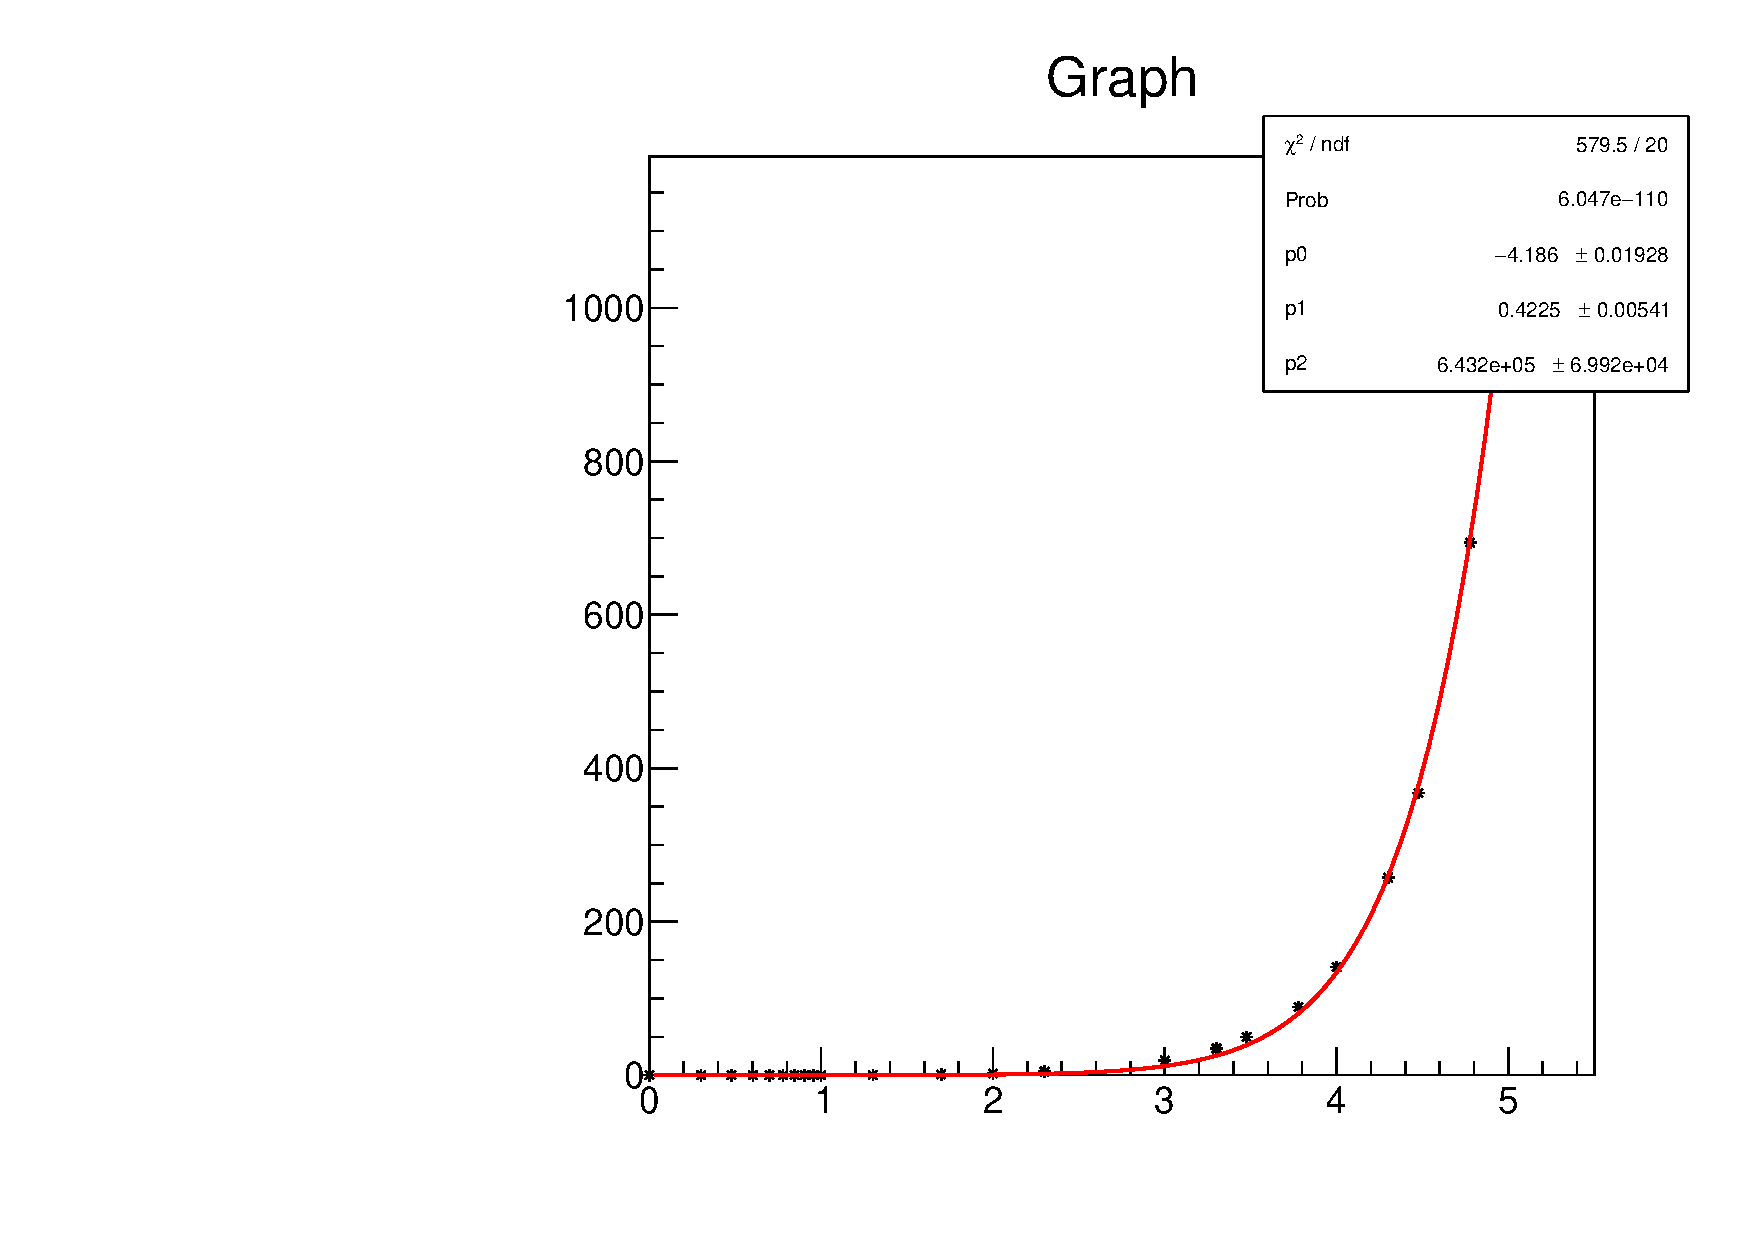
\includegraphics[width=0.6\textwidth]{figs/ata03/20250921/1758456926.pdf}
  \caption{ミューオン発生数のエネルギー依存性}
  \label{fig:cosmic_muon_flux}
\end{figure}
\begin{figure}
  \centering
  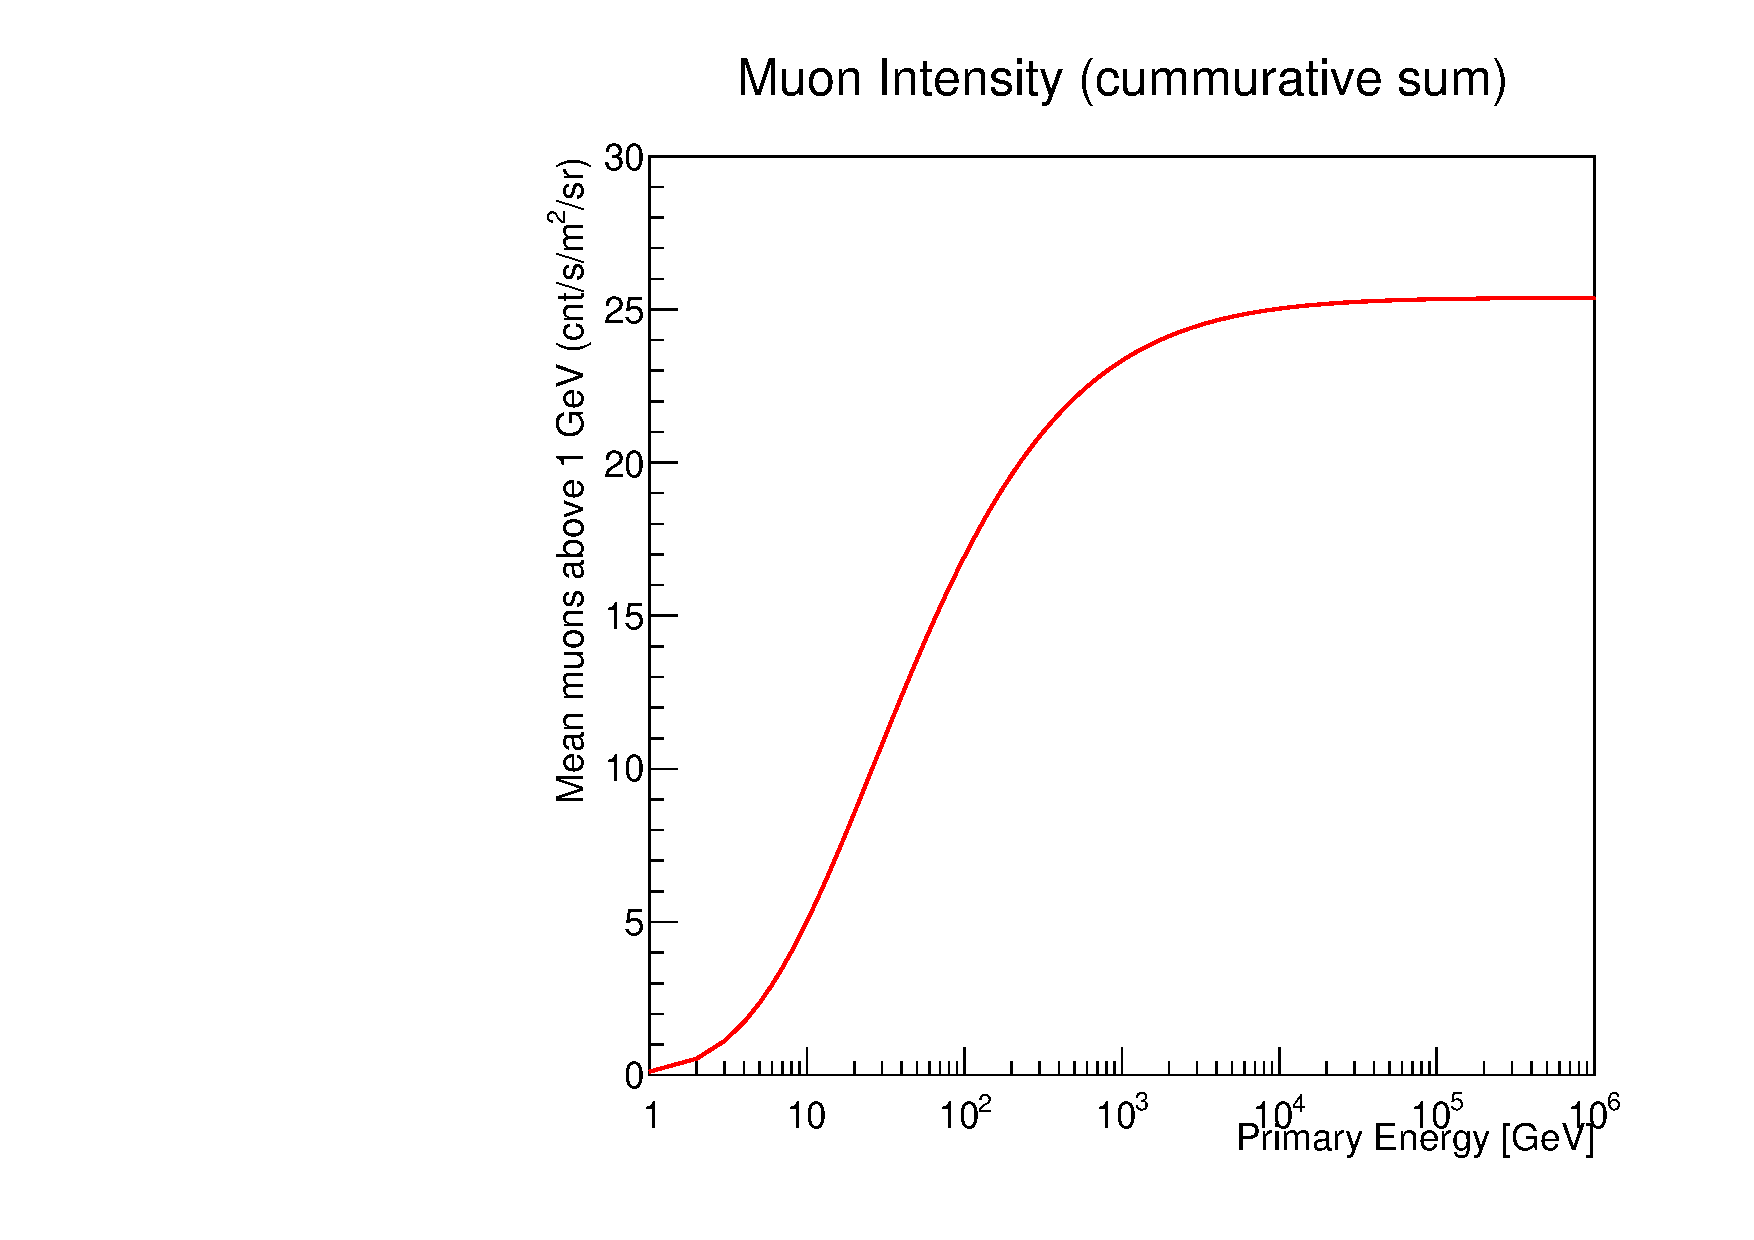
\includegraphics[width=0.6\textwidth]{figs/ata03/20250921/1758456906.pdf}
  \caption{ミューオン到来数の累積分布関数}
  \label{fig:cosmic_muon_flux}
\end{figure}

